\documentclass[twoside]{book}

% Packages required by doxygen
\usepackage{fixltx2e}
\usepackage{calc}
\usepackage{doxygen}
\usepackage[export]{adjustbox} % also loads graphicx
\usepackage{graphicx}
\usepackage[utf8]{inputenc}
\usepackage{makeidx}
\usepackage{multicol}
\usepackage{multirow}
\PassOptionsToPackage{warn}{textcomp}
\usepackage{textcomp}
\usepackage[nointegrals]{wasysym}
\usepackage[table]{xcolor}

% Font selection
\usepackage[T1]{fontenc}
\usepackage[scaled=.90]{helvet}
\usepackage{courier}
\usepackage{amssymb}
\usepackage{sectsty}
\renewcommand{\familydefault}{\sfdefault}
\allsectionsfont{%
  \fontseries{bc}\selectfont%
  \color{darkgray}%
}
\renewcommand{\DoxyLabelFont}{%
  \fontseries{bc}\selectfont%
  \color{darkgray}%
}
\newcommand{\+}{\discretionary{\mbox{\scriptsize$\hookleftarrow$}}{}{}}

% Page & text layout
\usepackage{geometry}
\geometry{%
  a4paper,%
  top=2.5cm,%
  bottom=2.5cm,%
  left=2.5cm,%
  right=2.5cm%
}
\tolerance=750
\hfuzz=15pt
\hbadness=750
\setlength{\emergencystretch}{15pt}
\setlength{\parindent}{0cm}
\setlength{\parskip}{3ex plus 2ex minus 2ex}
\makeatletter
\renewcommand{\paragraph}{%
  \@startsection{paragraph}{4}{0ex}{-1.0ex}{1.0ex}{%
    \normalfont\normalsize\bfseries\SS@parafont%
  }%
}
\renewcommand{\subparagraph}{%
  \@startsection{subparagraph}{5}{0ex}{-1.0ex}{1.0ex}{%
    \normalfont\normalsize\bfseries\SS@subparafont%
  }%
}
\makeatother

% Headers & footers
\usepackage{fancyhdr}
\pagestyle{fancyplain}
\fancyhead[LE]{\fancyplain{}{\bfseries\thepage}}
\fancyhead[CE]{\fancyplain{}{}}
\fancyhead[RE]{\fancyplain{}{\bfseries\leftmark}}
\fancyhead[LO]{\fancyplain{}{\bfseries\rightmark}}
\fancyhead[CO]{\fancyplain{}{}}
\fancyhead[RO]{\fancyplain{}{\bfseries\thepage}}
\fancyfoot[LE]{\fancyplain{}{}}
\fancyfoot[CE]{\fancyplain{}{}}
\fancyfoot[RE]{\fancyplain{}{\bfseries\scriptsize Generated by Doxygen }}
\fancyfoot[LO]{\fancyplain{}{\bfseries\scriptsize Generated by Doxygen }}
\fancyfoot[CO]{\fancyplain{}{}}
\fancyfoot[RO]{\fancyplain{}{}}
\renewcommand{\footrulewidth}{0.4pt}
\renewcommand{\chaptermark}[1]{%
  \markboth{#1}{}%
}
\renewcommand{\sectionmark}[1]{%
  \markright{\thesection\ #1}%
}

% Indices & bibliography
\usepackage{natbib}
\usepackage[titles]{tocloft}
\setcounter{tocdepth}{3}
\setcounter{secnumdepth}{5}
\makeindex

% Hyperlinks (required, but should be loaded last)
\usepackage{ifpdf}
\ifpdf
  \usepackage[pdftex,pagebackref=true]{hyperref}
\else
  \usepackage[ps2pdf,pagebackref=true]{hyperref}
\fi
\hypersetup{%
  colorlinks=true,%
  linkcolor=blue,%
  citecolor=blue,%
  unicode%
}

% Custom commands
\newcommand{\clearemptydoublepage}{%
  \newpage{\pagestyle{empty}\cleardoublepage}%
}

\usepackage{caption}
\captionsetup{labelsep=space,justification=centering,font={bf},singlelinecheck=off,skip=4pt,position=top}

%===== C O N T E N T S =====

\begin{document}

% Titlepage & ToC
\hypersetup{pageanchor=false,
             bookmarksnumbered=true,
             pdfencoding=unicode
            }
\pagenumbering{alph}
\begin{titlepage}
\vspace*{7cm}
\begin{center}%
{\Large My Project }\\
\vspace*{1cm}
{\large Generated by Doxygen 1.8.14}\\
\end{center}
\end{titlepage}
\clearemptydoublepage
\pagenumbering{roman}
\tableofcontents
\clearemptydoublepage
\pagenumbering{arabic}
\hypersetup{pageanchor=true}

%--- Begin generated contents ---
\chapter{Hierarchical Index}
\section{Class Hierarchy}
This inheritance list is sorted roughly, but not completely, alphabetically\+:\begin{DoxyCompactList}
\item \contentsline{section}{Employee}{\pageref{class_employee}}{}
\begin{DoxyCompactList}
\item \contentsline{section}{Commission\+Employee}{\pageref{class_commission_employee}}{}
\begin{DoxyCompactList}
\item \contentsline{section}{Base\+Plus\+Commission\+Employee}{\pageref{class_base_plus_commission_employee}}{}
\end{DoxyCompactList}
\item \contentsline{section}{Salaried\+Employee}{\pageref{class_salaried_employee}}{}
\end{DoxyCompactList}
\end{DoxyCompactList}

\chapter{Class Index}
\section{Class List}
Here are the classes, structs, unions and interfaces with brief descriptions\+:\begin{DoxyCompactList}
\item\contentsline{section}{\mbox{\hyperlink{class_base_plus_commission_employee}{Base\+Plus\+Commission\+Employee}} }{\pageref{class_base_plus_commission_employee}}{}
\item\contentsline{section}{\mbox{\hyperlink{class_commission_employee}{Commission\+Employee}} }{\pageref{class_commission_employee}}{}
\item\contentsline{section}{\mbox{\hyperlink{class_employee}{Employee}} }{\pageref{class_employee}}{}
\item\contentsline{section}{\mbox{\hyperlink{class_salaried_employee}{Salaried\+Employee}} }{\pageref{class_salaried_employee}}{}
\end{DoxyCompactList}

\chapter{Class Documentation}
\hypertarget{class_base_plus_commission_employee}{}\section{Base\+Plus\+Commission\+Employee Class Reference}
\label{class_base_plus_commission_employee}\index{Base\+Plus\+Commission\+Employee@{Base\+Plus\+Commission\+Employee}}


{\ttfamily \#include $<$Base\+Plus\+Commission\+Employee.\+h$>$}

Inheritance diagram for Base\+Plus\+Commission\+Employee\+:\begin{figure}[H]
\begin{center}
\leavevmode
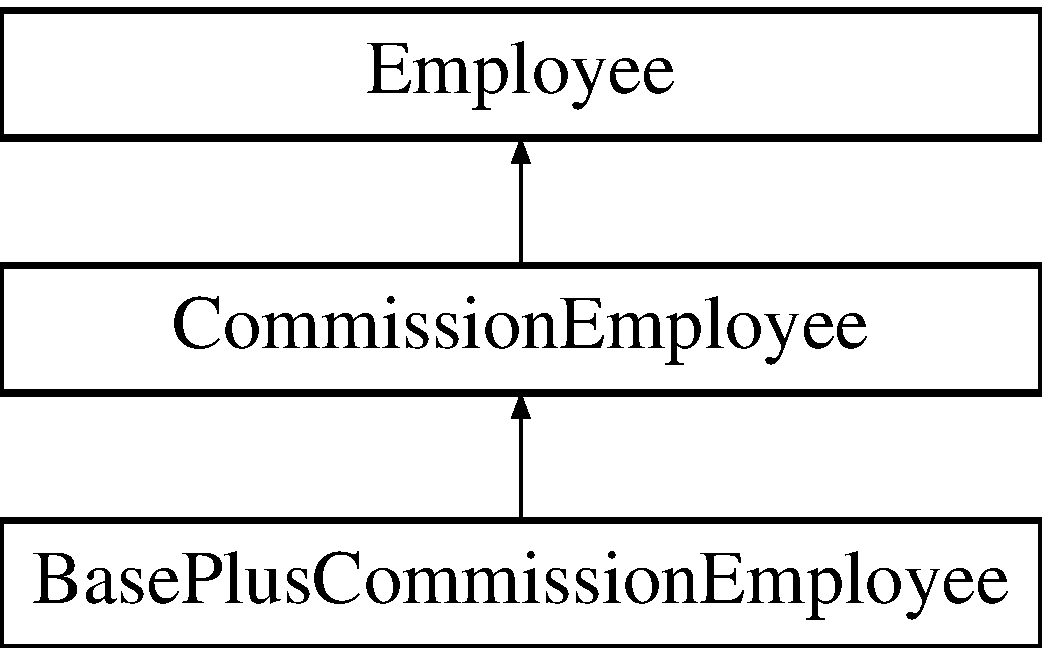
\includegraphics[height=3.000000cm]{class_base_plus_commission_employee}
\end{center}
\end{figure}
\subsection*{Public Member Functions}
\begin{DoxyCompactItemize}
\item 
\mbox{\Hypertarget{class_base_plus_commission_employee_a5648553e7a5a8337ae6cd6d0c5660e8a}\label{class_base_plus_commission_employee_a5648553e7a5a8337ae6cd6d0c5660e8a}} 
{\bfseries Base\+Plus\+Commission\+Employee} (const std\+::string \&, const std\+::string \&, const std\+::string \&, double=0.\+0, double=0.\+0, double=0.\+0)
\item 
\mbox{\Hypertarget{class_base_plus_commission_employee_a251fb6a98d7d9f427456fba0d0eaeeb1}\label{class_base_plus_commission_employee_a251fb6a98d7d9f427456fba0d0eaeeb1}} 
virtual \mbox{\hyperlink{class_base_plus_commission_employee_a251fb6a98d7d9f427456fba0d0eaeeb1}{$\sim$\+Base\+Plus\+Commission\+Employee}} ()=default
\begin{DoxyCompactList}\small\item\em virtual destructor \end{DoxyCompactList}\item 
\mbox{\Hypertarget{class_base_plus_commission_employee_aa66aca9c0d08a445942bbe4d9207c170}\label{class_base_plus_commission_employee_aa66aca9c0d08a445942bbe4d9207c170}} 
void \mbox{\hyperlink{class_base_plus_commission_employee_aa66aca9c0d08a445942bbe4d9207c170}{set\+Base\+Salary}} (double)
\begin{DoxyCompactList}\small\item\em set base salary \end{DoxyCompactList}\item 
\mbox{\Hypertarget{class_base_plus_commission_employee_a836f52adf74e6561b746a4330cb34c44}\label{class_base_plus_commission_employee_a836f52adf74e6561b746a4330cb34c44}} 
double \mbox{\hyperlink{class_base_plus_commission_employee_a836f52adf74e6561b746a4330cb34c44}{get\+Base\+Salary}} () const
\begin{DoxyCompactList}\small\item\em return base salary \end{DoxyCompactList}\item 
virtual double \mbox{\hyperlink{class_base_plus_commission_employee_a79cefc4722f05de0e545c2f911e2dcab}{earnings}} () const override
\begin{DoxyCompactList}\small\item\em keyword virtual signals intent to override \end{DoxyCompactList}\item 
\mbox{\Hypertarget{class_base_plus_commission_employee_a3e13b88007de250004e95864999cb591}\label{class_base_plus_commission_employee_a3e13b88007de250004e95864999cb591}} 
virtual std\+::string \mbox{\hyperlink{class_base_plus_commission_employee_a3e13b88007de250004e95864999cb591}{to\+String}} () const override
\begin{DoxyCompactList}\small\item\em string representation \end{DoxyCompactList}\end{DoxyCompactItemize}


\subsection{Detailed Description}
Fig. 12.\+15\+: \mbox{\hyperlink{_base_plus_commission_employee_8h_source}{Base\+Plus\+Commission\+Employee.\+h}}. \mbox{\hyperlink{class_base_plus_commission_employee}{Base\+Plus\+Commission\+Employee}} class derived from \mbox{\hyperlink{class_commission_employee}{Commission\+Employee}}. 

\subsection{Member Function Documentation}
\mbox{\Hypertarget{class_base_plus_commission_employee_a79cefc4722f05de0e545c2f911e2dcab}\label{class_base_plus_commission_employee_a79cefc4722f05de0e545c2f911e2dcab}} 
\index{Base\+Plus\+Commission\+Employee@{Base\+Plus\+Commission\+Employee}!earnings@{earnings}}
\index{earnings@{earnings}!Base\+Plus\+Commission\+Employee@{Base\+Plus\+Commission\+Employee}}
\subsubsection{\texorpdfstring{earnings()}{earnings()}}
{\footnotesize\ttfamily double Base\+Plus\+Commission\+Employee\+::earnings (\begin{DoxyParamCaption}{ }\end{DoxyParamCaption}) const\hspace{0.3cm}{\ttfamily [override]}, {\ttfamily [virtual]}}



keyword virtual signals intent to override 

calculate earnings 

Reimplemented from \mbox{\hyperlink{class_commission_employee_aa7759d5908bd7357a9976c2c2740e9bb}{Commission\+Employee}}.



The documentation for this class was generated from the following files\+:\begin{DoxyCompactItemize}
\item 
Base\+Plus\+Commission\+Employee.\+h\item 
Base\+Plus\+Commission\+Employee.\+cpp\end{DoxyCompactItemize}

\hypertarget{class_commission_employee}{}\section{Commission\+Employee Class Reference}
\label{class_commission_employee}\index{Commission\+Employee@{Commission\+Employee}}


{\ttfamily \#include $<$Commission\+Employee.\+h$>$}

Inheritance diagram for Commission\+Employee\+:\begin{figure}[H]
\begin{center}
\leavevmode
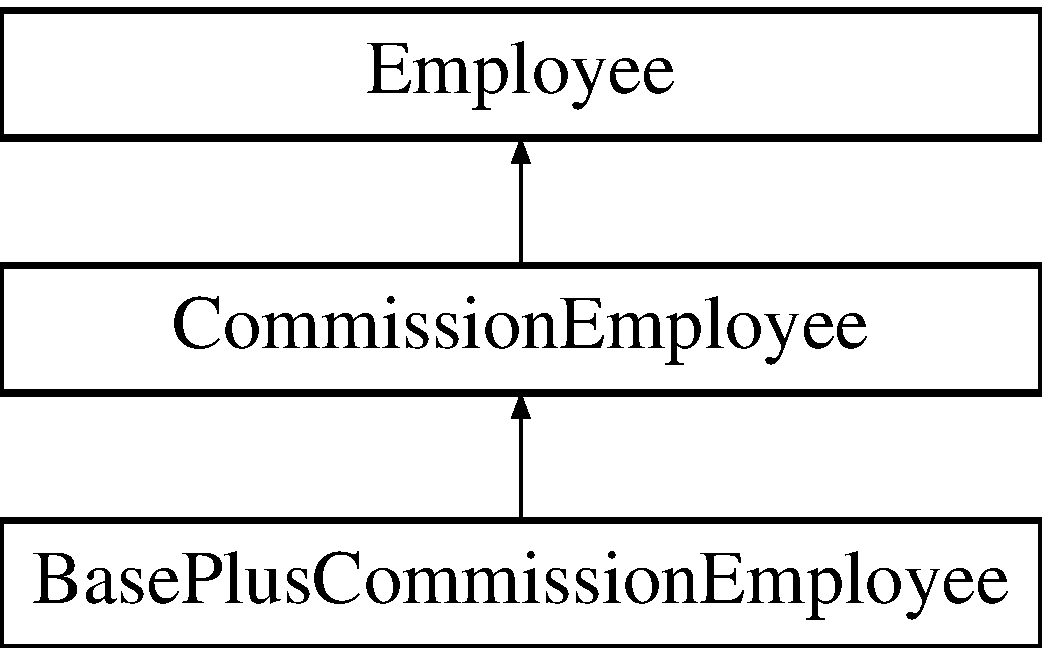
\includegraphics[height=3.000000cm]{class_commission_employee}
\end{center}
\end{figure}
\subsection*{Public Member Functions}
\begin{DoxyCompactItemize}
\item 
\mbox{\Hypertarget{class_commission_employee_a46ccb62795b2c82b2ce5d9ca109d21af}\label{class_commission_employee_a46ccb62795b2c82b2ce5d9ca109d21af}} 
{\bfseries Commission\+Employee} (const std\+::string \&, const std\+::string \&, const std\+::string \&, double=0.\+0, double=0.\+0)
\item 
\mbox{\Hypertarget{class_commission_employee_a85d35440afb6065ed90982165bd8a45e}\label{class_commission_employee_a85d35440afb6065ed90982165bd8a45e}} 
virtual \mbox{\hyperlink{class_commission_employee_a85d35440afb6065ed90982165bd8a45e}{$\sim$\+Commission\+Employee}} ()=default
\begin{DoxyCompactList}\small\item\em virtual destructor \end{DoxyCompactList}\item 
\mbox{\Hypertarget{class_commission_employee_a9604cfc3151934d2c5616f6961e0abe6}\label{class_commission_employee_a9604cfc3151934d2c5616f6961e0abe6}} 
void \mbox{\hyperlink{class_commission_employee_a9604cfc3151934d2c5616f6961e0abe6}{set\+Commission\+Rate}} (double)
\begin{DoxyCompactList}\small\item\em set commission rate \end{DoxyCompactList}\item 
\mbox{\Hypertarget{class_commission_employee_a494b60111ebada810df48421fe57f875}\label{class_commission_employee_a494b60111ebada810df48421fe57f875}} 
double \mbox{\hyperlink{class_commission_employee_a494b60111ebada810df48421fe57f875}{get\+Commission\+Rate}} () const
\begin{DoxyCompactList}\small\item\em return commission rate \end{DoxyCompactList}\item 
\mbox{\Hypertarget{class_commission_employee_a28a54096a9fd1468c39dc03a7f14e543}\label{class_commission_employee_a28a54096a9fd1468c39dc03a7f14e543}} 
void \mbox{\hyperlink{class_commission_employee_a28a54096a9fd1468c39dc03a7f14e543}{set\+Gross\+Sales}} (double)
\begin{DoxyCompactList}\small\item\em set gross sales amount \end{DoxyCompactList}\item 
\mbox{\Hypertarget{class_commission_employee_acafd14323207ade77db368b050be9376}\label{class_commission_employee_acafd14323207ade77db368b050be9376}} 
double \mbox{\hyperlink{class_commission_employee_acafd14323207ade77db368b050be9376}{get\+Gross\+Sales}} () const
\begin{DoxyCompactList}\small\item\em return gross sales amount \end{DoxyCompactList}\item 
virtual double \mbox{\hyperlink{class_commission_employee_aa7759d5908bd7357a9976c2c2740e9bb}{earnings}} () const override
\begin{DoxyCompactList}\small\item\em keyword virtual signals intent to override \end{DoxyCompactList}\item 
\mbox{\Hypertarget{class_commission_employee_a9b0a2adfd93e4df96236b1e1758596f9}\label{class_commission_employee_a9b0a2adfd93e4df96236b1e1758596f9}} 
virtual std\+::string \mbox{\hyperlink{class_commission_employee_a9b0a2adfd93e4df96236b1e1758596f9}{to\+String}} () const override
\begin{DoxyCompactList}\small\item\em string representation \end{DoxyCompactList}\end{DoxyCompactItemize}


\subsection{Detailed Description}
Fig. 12.\+13\+: \mbox{\hyperlink{_commission_employee_8h_source}{Commission\+Employee.\+h}} \mbox{\hyperlink{class_commission_employee}{Commission\+Employee}} class derived from \mbox{\hyperlink{class_employee}{Employee}}. 

\subsection{Member Function Documentation}
\mbox{\Hypertarget{class_commission_employee_aa7759d5908bd7357a9976c2c2740e9bb}\label{class_commission_employee_aa7759d5908bd7357a9976c2c2740e9bb}} 
\index{Commission\+Employee@{Commission\+Employee}!earnings@{earnings}}
\index{earnings@{earnings}!Commission\+Employee@{Commission\+Employee}}
\subsubsection{\texorpdfstring{earnings()}{earnings()}}
{\footnotesize\ttfamily double Commission\+Employee\+::earnings (\begin{DoxyParamCaption}{ }\end{DoxyParamCaption}) const\hspace{0.3cm}{\ttfamily [override]}, {\ttfamily [virtual]}}



keyword virtual signals intent to override 

calculate earnings 

Implements \mbox{\hyperlink{class_employee_a821a8bea1db657efc004670c8481cbae}{Employee}}.



Reimplemented in \mbox{\hyperlink{class_base_plus_commission_employee_a79cefc4722f05de0e545c2f911e2dcab}{Base\+Plus\+Commission\+Employee}}.



The documentation for this class was generated from the following files\+:\begin{DoxyCompactItemize}
\item 
Commission\+Employee.\+h\item 
Commission\+Employee.\+cpp\end{DoxyCompactItemize}

\hypertarget{class_employee}{}\section{Employee Class Reference}
\label{class_employee}\index{Employee@{Employee}}


{\ttfamily \#include $<$Employee.\+h$>$}

Inheritance diagram for Employee\+:\begin{figure}[H]
\begin{center}
\leavevmode
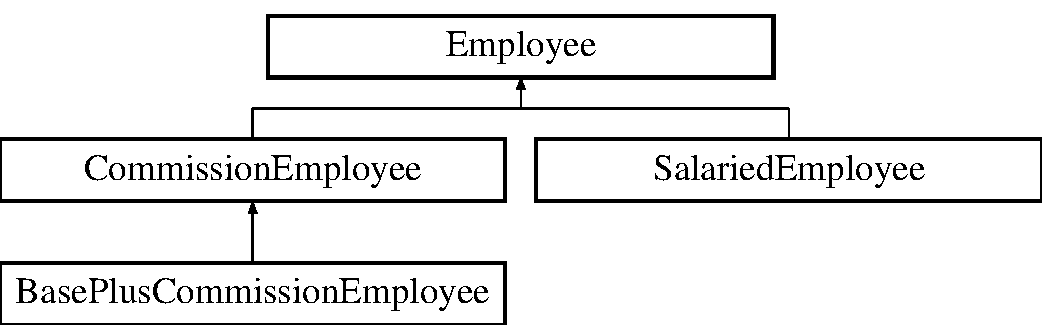
\includegraphics[height=3.000000cm]{class_employee}
\end{center}
\end{figure}
\subsection*{Public Member Functions}
\begin{DoxyCompactItemize}
\item 
\mbox{\Hypertarget{class_employee_aea37f8ab922dd5c4e4e033506efe4ad8}\label{class_employee_aea37f8ab922dd5c4e4e033506efe4ad8}} 
{\bfseries Employee} (const std\+::string \&, const std\+::string \&, const std\+::string \&)
\item 
\mbox{\Hypertarget{class_employee_a01aa009d0ef6b36afdc4aea4da1123a1}\label{class_employee_a01aa009d0ef6b36afdc4aea4da1123a1}} 
virtual \mbox{\hyperlink{class_employee_a01aa009d0ef6b36afdc4aea4da1123a1}{$\sim$\+Employee}} ()=default
\begin{DoxyCompactList}\small\item\em compiler generates virtual destructor \end{DoxyCompactList}\item 
\mbox{\Hypertarget{class_employee_a15e4ef686f54493b5afe52497000675e}\label{class_employee_a15e4ef686f54493b5afe52497000675e}} 
void \mbox{\hyperlink{class_employee_a15e4ef686f54493b5afe52497000675e}{set\+First\+Name}} (const std\+::string \&)
\begin{DoxyCompactList}\small\item\em set first name \end{DoxyCompactList}\item 
\mbox{\Hypertarget{class_employee_aef7422ec385231d030f1bf3f53d8563b}\label{class_employee_aef7422ec385231d030f1bf3f53d8563b}} 
std\+::string \mbox{\hyperlink{class_employee_aef7422ec385231d030f1bf3f53d8563b}{get\+First\+Name}} () const
\begin{DoxyCompactList}\small\item\em return first name \end{DoxyCompactList}\item 
\mbox{\Hypertarget{class_employee_a784d4bd99607405393f46e8648008a42}\label{class_employee_a784d4bd99607405393f46e8648008a42}} 
void \mbox{\hyperlink{class_employee_a784d4bd99607405393f46e8648008a42}{set\+Last\+Name}} (const std\+::string \&)
\begin{DoxyCompactList}\small\item\em set last name \end{DoxyCompactList}\item 
\mbox{\Hypertarget{class_employee_a9a9e3d0c77c609e5016589926844b003}\label{class_employee_a9a9e3d0c77c609e5016589926844b003}} 
std\+::string \mbox{\hyperlink{class_employee_a9a9e3d0c77c609e5016589926844b003}{get\+Last\+Name}} () const
\begin{DoxyCompactList}\small\item\em return last name \end{DoxyCompactList}\item 
\mbox{\Hypertarget{class_employee_a981082b8cf7727af8fbff6291dd03bee}\label{class_employee_a981082b8cf7727af8fbff6291dd03bee}} 
void \mbox{\hyperlink{class_employee_a981082b8cf7727af8fbff6291dd03bee}{set\+Social\+Security\+Number}} (const std\+::string \&)
\begin{DoxyCompactList}\small\item\em set S\+SN \end{DoxyCompactList}\item 
\mbox{\Hypertarget{class_employee_afe97463fcee4f5cbc6eb55914887789f}\label{class_employee_afe97463fcee4f5cbc6eb55914887789f}} 
std\+::string \mbox{\hyperlink{class_employee_afe97463fcee4f5cbc6eb55914887789f}{get\+Social\+Security\+Number}} () const
\begin{DoxyCompactList}\small\item\em return S\+SN \end{DoxyCompactList}\item 
virtual double \mbox{\hyperlink{class_employee_a821a8bea1db657efc004670c8481cbae}{earnings}} () const =0
\begin{DoxyCompactList}\small\item\em pure virtual function makes \mbox{\hyperlink{class_employee}{Employee}} an abstract base class \end{DoxyCompactList}\item 
\mbox{\Hypertarget{class_employee_aff7d34f5d6587ba947313b3bbce3e52d}\label{class_employee_aff7d34f5d6587ba947313b3bbce3e52d}} 
virtual std\+::string \mbox{\hyperlink{class_employee_aff7d34f5d6587ba947313b3bbce3e52d}{to\+String}} () const
\begin{DoxyCompactList}\small\item\em virtual \end{DoxyCompactList}\end{DoxyCompactItemize}


\subsection{Detailed Description}
Fig. 12.\+9\+: \mbox{\hyperlink{_employee_8h_source}{Employee.\+h}} \mbox{\hyperlink{class_employee}{Employee}} abstract base class. 

\subsection{Member Function Documentation}
\mbox{\Hypertarget{class_employee_a821a8bea1db657efc004670c8481cbae}\label{class_employee_a821a8bea1db657efc004670c8481cbae}} 
\index{Employee@{Employee}!earnings@{earnings}}
\index{earnings@{earnings}!Employee@{Employee}}
\subsubsection{\texorpdfstring{earnings()}{earnings()}}
{\footnotesize\ttfamily virtual double Employee\+::earnings (\begin{DoxyParamCaption}{ }\end{DoxyParamCaption}) const\hspace{0.3cm}{\ttfamily [pure virtual]}}



pure virtual function makes \mbox{\hyperlink{class_employee}{Employee}} an abstract base class 

pure virtual 

Implemented in \mbox{\hyperlink{class_commission_employee_aa7759d5908bd7357a9976c2c2740e9bb}{Commission\+Employee}}, \mbox{\hyperlink{class_salaried_employee_a917d254c8869beb7a3c1f1d0787b1515}{Salaried\+Employee}}, and \mbox{\hyperlink{class_base_plus_commission_employee_a79cefc4722f05de0e545c2f911e2dcab}{Base\+Plus\+Commission\+Employee}}.



The documentation for this class was generated from the following files\+:\begin{DoxyCompactItemize}
\item 
Employee.\+h\item 
Employee.\+cpp\end{DoxyCompactItemize}

\hypertarget{class_salaried_employee}{}\section{Salaried\+Employee Class Reference}
\label{class_salaried_employee}\index{Salaried\+Employee@{Salaried\+Employee}}


{\ttfamily \#include $<$Salaried\+Employee.\+h$>$}

Inheritance diagram for Salaried\+Employee\+:\begin{figure}[H]
\begin{center}
\leavevmode
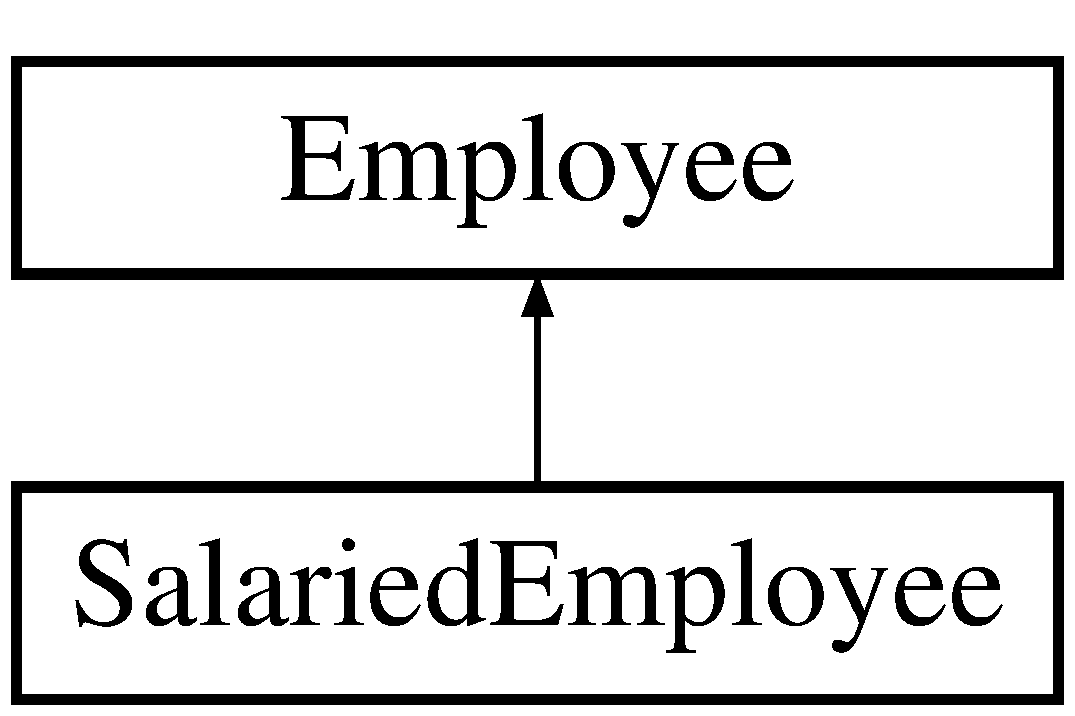
\includegraphics[height=2.000000cm]{class_salaried_employee}
\end{center}
\end{figure}
\subsection*{Public Member Functions}
\begin{DoxyCompactItemize}
\item 
\mbox{\Hypertarget{class_salaried_employee_a4d418f4de5381b4e0af8848013bbb449}\label{class_salaried_employee_a4d418f4de5381b4e0af8848013bbb449}} 
{\bfseries Salaried\+Employee} (const std\+::string \&, const std\+::string \&, const std\+::string \&, double=0.\+0)
\item 
\mbox{\Hypertarget{class_salaried_employee_a718d71a5880188902a040e2509a759b8}\label{class_salaried_employee_a718d71a5880188902a040e2509a759b8}} 
virtual \mbox{\hyperlink{class_salaried_employee_a718d71a5880188902a040e2509a759b8}{$\sim$\+Salaried\+Employee}} ()=default
\begin{DoxyCompactList}\small\item\em virtual destructor \end{DoxyCompactList}\item 
\mbox{\Hypertarget{class_salaried_employee_a97b0a3186e6d2bd3f42f4dd171795dfa}\label{class_salaried_employee_a97b0a3186e6d2bd3f42f4dd171795dfa}} 
void \mbox{\hyperlink{class_salaried_employee_a97b0a3186e6d2bd3f42f4dd171795dfa}{set\+Weekly\+Salary}} (double)
\begin{DoxyCompactList}\small\item\em set weekly salary \end{DoxyCompactList}\item 
\mbox{\Hypertarget{class_salaried_employee_a9990ee16056641bf697c030e9e5591a6}\label{class_salaried_employee_a9990ee16056641bf697c030e9e5591a6}} 
double \mbox{\hyperlink{class_salaried_employee_a9990ee16056641bf697c030e9e5591a6}{get\+Weekly\+Salary}} () const
\begin{DoxyCompactList}\small\item\em return weekly salary \end{DoxyCompactList}\item 
\mbox{\Hypertarget{class_salaried_employee_a917d254c8869beb7a3c1f1d0787b1515}\label{class_salaried_employee_a917d254c8869beb7a3c1f1d0787b1515}} 
virtual double \mbox{\hyperlink{class_salaried_employee_a917d254c8869beb7a3c1f1d0787b1515}{earnings}} () const override
\begin{DoxyCompactList}\small\item\em calculate earnings \end{DoxyCompactList}\item 
\mbox{\Hypertarget{class_salaried_employee_a4e23874945c70228e93f9883399c0909}\label{class_salaried_employee_a4e23874945c70228e93f9883399c0909}} 
virtual std\+::string \mbox{\hyperlink{class_salaried_employee_a4e23874945c70228e93f9883399c0909}{to\+String}} () const override
\begin{DoxyCompactList}\small\item\em string representation \end{DoxyCompactList}\end{DoxyCompactItemize}


\subsection{Detailed Description}
Fig. 12.\+11\+: \mbox{\hyperlink{_salaried_employee_8h_source}{Salaried\+Employee.\+h}} \mbox{\hyperlink{class_salaried_employee}{Salaried\+Employee}} class derived from \mbox{\hyperlink{class_employee}{Employee}}. 

The documentation for this class was generated from the following files\+:\begin{DoxyCompactItemize}
\item 
Salaried\+Employee.\+h\item 
Salaried\+Employee.\+cpp\end{DoxyCompactItemize}

%--- End generated contents ---

% Index
\backmatter
\newpage
\phantomsection
\clearemptydoublepage
\addcontentsline{toc}{chapter}{Index}
\printindex

\end{document}
